\chapter{Лекция 6. Гамильтоновы графы. Графы де Брёйна. Деревья}

% ============================================================
% ГАМИЛЬТОНОВЫ ГРАФЫ (стр. 15, dir2 стр. 3)
% ============================================================

\subsection*{Гамильтоновы графы}

\begin{defn}{Гамильтонов путь}{hamilton-path}
$G(V, E)$.

$G$ содержит \textbf{гамильтонов путь} $\;\Leftrightarrow\;$ $\exists$ путь, проходящий через
$\forall\, v \in V$ ровно 1 раз.

$\Rightarrow\;$ $G$ --- \textbf{полугамильтонов}.
\end{defn}

\begin{defn}{Гамильтонов цикл}{hamilton-cycle}
$G$ содержит \textbf{гамильтонов цикл} $\;\Leftrightarrow\;$ $\exists$ замкнутый простой путь через
$\forall\, v \in V$ ровно 1 раз, кроме $v_{\text{start}} = v_{\text{finish}}$.

$\Rightarrow\;$ $G$ --- \textbf{гамильтонов}.
\end{defn}

\medskip
\noindent\textbf{Примеры:}

% Пример 1: путь 1—2—3—4 — полугамильтонов
% Граф: p15-example-1.graph
\grfig{figures/p15-example-1.pdf}{Полугамильтонов: цепь $1$--$2$--$3$--$4$}
\noindent\textit{Пример 1.} Цепь $1$--$2$--$3$--$4$ сама является гамильтоновым
путём (каждая вершина ровно один раз), но цикла нет --- граф
\textbf{полугамильтонов}.

% Пример 2: цикл 1—2—3—4—1 — гамильтонов (и полугамильтонов)
% Граф: p15-example-2.graph
\grfig{figures/p15-example-2.pdf}{Гамильтонов (и полугамильтонов): цикл $1$--$2$--$3$--$4$--$1$}
\noindent\textit{Пример 2.} Цикл $1$--$2$--$3$--$4$--$1$ --- гамильтонов цикл,
поэтому граф \textbf{гамильтонов} (а значит, и \textbf{полугамильтонов}:
убрав последнее ребро цикла, получаем гамильтонов путь).

% Пример 3: 1—2—3, 2—4 (звезда) — ни гам., ни полугам.
% Граф: p15-example-3.graph
\grfig{figures/p15-example-3.pdf}{Ни гамильтонов, ни полугамильтонов: $1$--$2$--$3$, $2$--$4$}
\noindent\textit{Пример 3.} <<Звезда>> $1$--$2$--$3$ c дополнительным листом
$2$--$4$: любой путь, заходящий во все три листа $1, 3, 4$, обязан
проходить через центр $2$ минимум дважды --- граф \textbf{ни гамильтонов,
ни полугамильтонов}.

\medskip
\textbf{Замечание.} Теоремы ниже дают только \emph{достаточные} условия
гамильтоновости: если условие выполнено --- граф точно гамильтонов, но если
условие \emph{не} выполнено, это ещё не значит, что граф не гамильтонов
(например, цикл $C_5$ гамильтонов, хотя все степени равны $2 < 5/2$).

\medskip
Условия гамильтоновости ($G(V,E)$ --- неориент., связный):

\begin{statement}{Теорема Оре}{ore}
$|V| = n \ge 3$. Если $\forall\, u, v \in V$ т.\,ч. $\nexists\, e = uv$
\textup{($u, v$ --- несмежные)}:
$\deg(u) + \deg(v) \geq n$,
то $G$ --- гамильтонов.
\end{statement}

\begin{proof}
От противного. Пусть условие выполнено, но гамильтонова цикла нет. Будем
добавлять в $G$ рёбра, пока это возможно без появления гамильтонова цикла
(условие Оре при добавлении рёбер тем более сохраняется); получим
\emph{максимальный} контрпример $G'$: гамильтонова цикла нет, но
добавление любого ребра его создаёт.

В $G'$ есть несмежные вершины $u, v$ (иначе $G' = K_n$ --- гамильтонов).
Добавление ребра $uv$ создаёт гамильтонов цикл, значит уже в $G'$ есть
гамильтонов \emph{путь} $u = v_1, v_2, \ldots, v_n = v$.

Рассмотрим множества индексов
$S = \{\, i \mid u \sim v_{i+1} \,\}$ и $T = \{\, i \mid v \sim v_i \,\}$;
$|S| = \deg(u)$, $|T| = \deg(v)$, причём $S, T \subseteq \{1, \dots, n-1\}$.
Так как $|S| + |T| = \deg(u) + \deg(v) \ge n > n - 1$, по принципу Дирихле
$\exists\, i \in S \cap T$: одновременно $u \sim v_{i+1}$ и $v \sim v_i$.
Тогда
\[
  u = v_1, v_2, \ldots, v_i,\; v_n = v,\; v_{n-1}, \ldots, v_{i+1},\; v_1
\]
--- гамильтонов цикл (идём по пути до $v_i$, прыгаем по ребру $v_i v_n$
в конец, возвращаемся по пути назад до $v_{i+1}$ и замыкаемся ребром
$v_{i+1} u$). Противоречие с тем, что в $G'$ цикла нет.
\end{proof}

\begin{statement}{Теорема Дирака}{dirac}
$|V| = n \ge 3$. Если $\forall\, u \in V$: $\deg(u) \geq \dfrac{n}{2}$,
то $G$ --- гамильтонов.
\end{statement}

\begin{proof}
Частный случай теоремы Оре: для любых несмежных $u, v$ имеем
$\deg(u) + \deg(v) \ge \frac{n}{2} + \frac{n}{2} = n$.
\end{proof}

\begin{defn}{Турнир}{tournament}
\textbf{Турнир} --- ориентированный граф, в котором каждая пара
различных вершин соединена \emph{ровно одной} дугой (в одном из двух
направлений). Иначе говоря, турнир --- это полный граф $K_n$, каждому
ребру которого приписана ориентация.
\end{defn}

\grfig[0.42]{figures/p15-tournament-1.pdf}{Турнир на 4 вершинах: гамильтонов путь $1 \to 2 \to 3 \to 4$}

\textbf{Примеры.} 1) Результаты кругового спортивного турнира без
ничьих: вершины --- участники, дуга $u \to v$ означает <<$u$ выиграл у
$v$>> (отсюда и название). На рисунке: $1$ победил всех, $4$ проиграл
всем, между $2$ и $3$ --- победа $2$. 2) Транзитивный турнир: вершины
$1, \ldots, n$, все дуги от меньшего номера к большему --- это в
точности строгий линейный порядок из лекции 3.

\begin{statement}{Теорема Редеи (о турнирах)}{redei}
В любом турнире существует гамильтонов путь.
\end{statement}

\begin{proof}
Индукция по числу вершин $n$. База $n = 1$ тривиальна. Переход: удалим
из турнира вершину $v$; на оставшихся $n - 1$ вершинах по предположению
индукции есть гамильтонов путь $u_1 \to u_2 \to \ldots \to u_{n-1}$.
Вставим $v$:
\begin{itemize}
  \item если $v \to u_1$ --- ставим $v$ в начало;
  \item иначе $u_1 \to v$; пусть $i$ --- наибольший индекс с
        $u_i \to v$. Если $i = n - 1$, ставим $v$ в конец. Если же
        $i < n - 1$, то по максимальности $v \to u_{i+1}$, и $v$
        вставляется между $u_i$ и $u_{i+1}$:
        $u_1 \to \ldots \to u_i \to v \to u_{i+1} \to \ldots \to u_{n-1}$.
\end{itemize}
В каждом случае получили гамильтонов путь на всех $n$ вершинах
(заметим: гамильтонов \emph{цикл} в турнире существовать не обязан ---
в транзитивном турнире из последней вершины дуги не выходят).
\end{proof}

% ============================================================
% Построение гамильтонова пути (в условиях т. Дирака)
% (стр. 15–16, dir2 стр. 3–4)
% ============================================================

\begin{algo}{Построение гамильтонова пути в условиях теоремы Дирака}{hamilton-dirac}

\textbf{Инициализация:} $v_1, v_2, \ldots, v_n$ --- произвольный порядок
\emph{всех} вершин графа.

\textbf{Шаг (поворот):} пока в последовательности есть несмежная соседняя
пара $(v_i, v_{i+1})$, ищем индекс $j > i + 1$, для которого
\emph{оба} ребра существуют:
\[
  \exists\, e_1 = v_i v_j \quad\text{и}\quad \exists\, e_2 = v_{i+1} v_{j+1};
\]
(условие Дирака гарантирует, что такой $j$ найдётся). Переворачиваем
отрезок $v_{i+1} \ldots v_j$:
\[
  v_1 \ldots v_i \;\bigl|\; \underbrace{v_j \, v_{j-1} \ldots v_{i+1}}_{\text{перевёрнут}} \;\bigl|\; v_{j+1} \ldots v_n.
\]
На стыках теперь стоят пары $(v_i, v_j)$ и $(v_{i+1}, v_{j+1})$ ---
обе смежные, а внутри перевёрнутого отрезка смежность пар не изменилась.
Число несмежных пар строго уменьшилось; повторяем, пока их не останется
--- получился гамильтонов путь.

\medskip
\noindent\textbf{Пример.} Возьмём граф с рёбрами
$A$--$C$, $C$--$E$, $E$--$F$, $F$--$D$, $D$--$B$, $B$--$A$, $A$--$D$,
$C$--$F$, $B$--$E$ (к графу с рис. выше по тексту добавлено ребро
$B$--$E$, чтобы выполнялось условие Дирака: теперь все степени равны
$3 = \frac{6}{2} = \frac{n}{2}$).

\grfig[0.5]{figures/p15-example-4b.pdf}{Алг. Дирака: граф $A,\dots,F$, все степени $= 3$}

Начальный порядок: $E, A, B, D, F, C$ --- т.\,е.
$v_1 = E,\; v_2 = A,\; v_3 = B,\; v_4 = D,\; v_5 = F,\; v_6 = C$.
Порядок \emph{произвольный} (алгоритм стартует с любого); этот выбран
для компактности примера --- в нём всего одна несмежная соседняя пара.
Проверяем пары: $(E, A)$ --- \emph{несмежная} (ребра $E$--$A$ нет);
остальные пары $(A,B), (B,D), (D,F), (F,C)$ --- смежные.

Чиним пару $(v_i, v_{i+1}) = (v_1, v_2) = (E, A)$. По описанию шага ищем
индекс $j > i + 1 = 2$, для которого существуют \emph{оба} ребра
$v_i v_j$ и $v_{i+1} v_{j+1}$, т.\,е. $E \sim v_j$ и $A \sim v_{j+1}$
--- перебираем кандидатов $j = 3, 4, 5$ по порядку:
\begin{itemize}
  \item $j = 3$: $v_3 = B$, $v_4 = D$. Проверяем: $E \sim B$? --- да
        (ребро $B$--$E$); $A \sim D$? --- да (ребро $A$--$D$).
        \textbf{Оба условия выполнены} --- берём $j = 3$ (дальше можно
        не перебирать; для сравнения: $j = 4$ не подошёл бы --- уже
        первое условие $E \sim v_4 = D$ не выполнено, ребра $E$--$D$
        в графе нет).
\end{itemize}
Переворачиваем отрезок $v_{i+1} \ldots v_j = v_2 \ldots v_3 = (A, B)$:
\[
  E,\; \underline{A,\; B},\; D,\; F,\; C
  \quad\longrightarrow\quad
  E,\; \underline{B,\; A},\; D,\; F,\; C.
\]
На стыках перевёрнутого отрезка встали проверенные рёбра: слева ---
$v_1 v_3 = E$--$B$, справа --- $v_2 v_4 = A$--$D$.
Все соседние пары теперь смежные: $E$--$B$, $B$--$A$, $A$--$D$, $D$--$F$,
$F$--$C$ --- это \textbf{гамильтонов путь}. Более того, концы $E$ и $C$
тоже смежны ($C$--$E$ --- ребро), так что путь замыкается в
\textbf{гамильтонов цикл} $E, B, A, D, F, C, E$.

\medskip
\noindent\textbf{Работа алгоритма по шагам} (синие рёбра --- смежные
соседние пары, красное --- несмежная пара, зелёные --- рёбра поворота
и итоговый путь):

\begin{center}\begin{tabular}{cc}
\shortstack{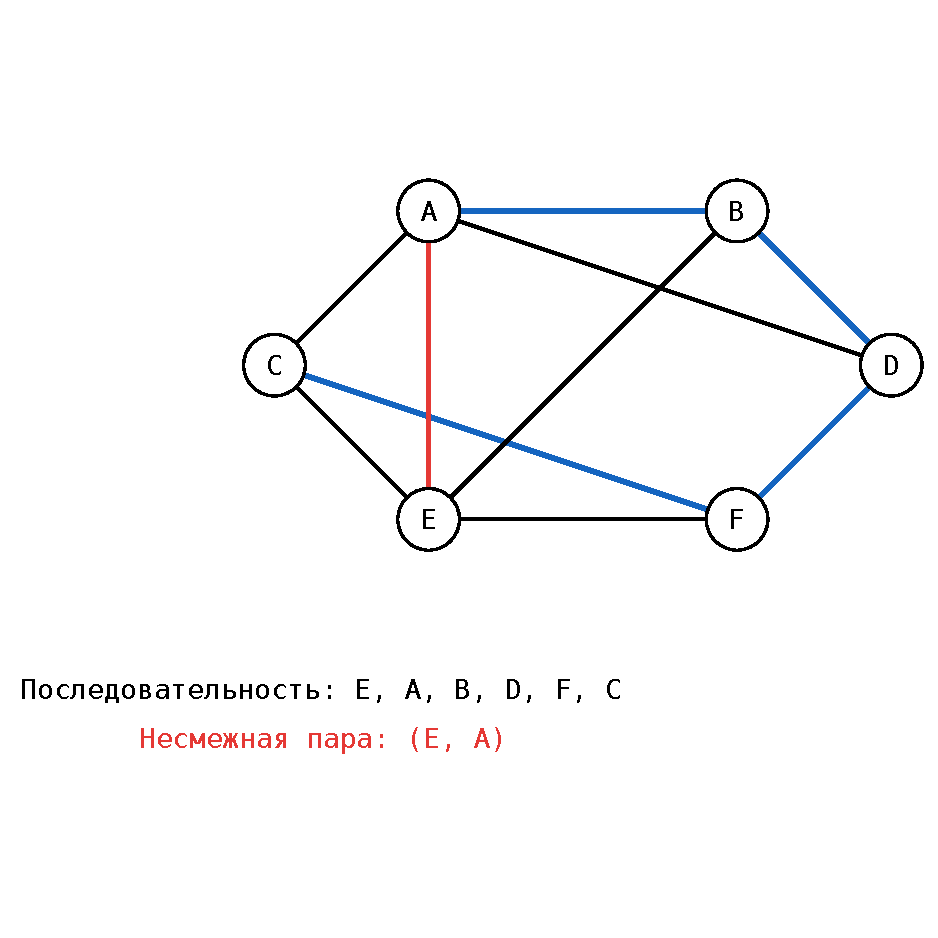
\includegraphics[width=0.46\textwidth]{python/lec06/hamilton/hamilton-0.pdf}\\[2pt]{\scriptsize Шаг 0. Порядок $E,A,B,D,F,C$; пара $(E,A)$ несмежная}} &
\shortstack{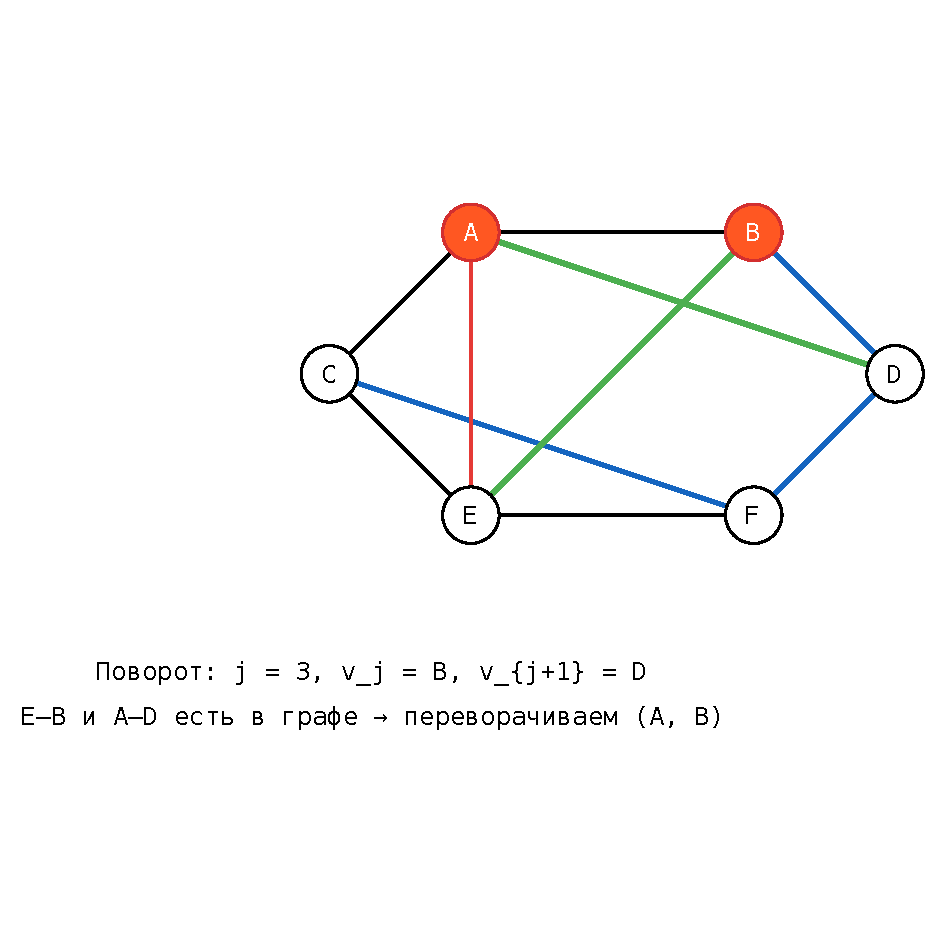
\includegraphics[width=0.46\textwidth]{python/lec06/hamilton/hamilton-1.pdf}\\[2pt]{\scriptsize Шаг 1. Поворот: $j=3$, рёбра $E$--$B$ и $A$--$D$ есть}} \\
\end{tabular}\end{center}
\begin{center}\begin{tabular}{cc}
\shortstack{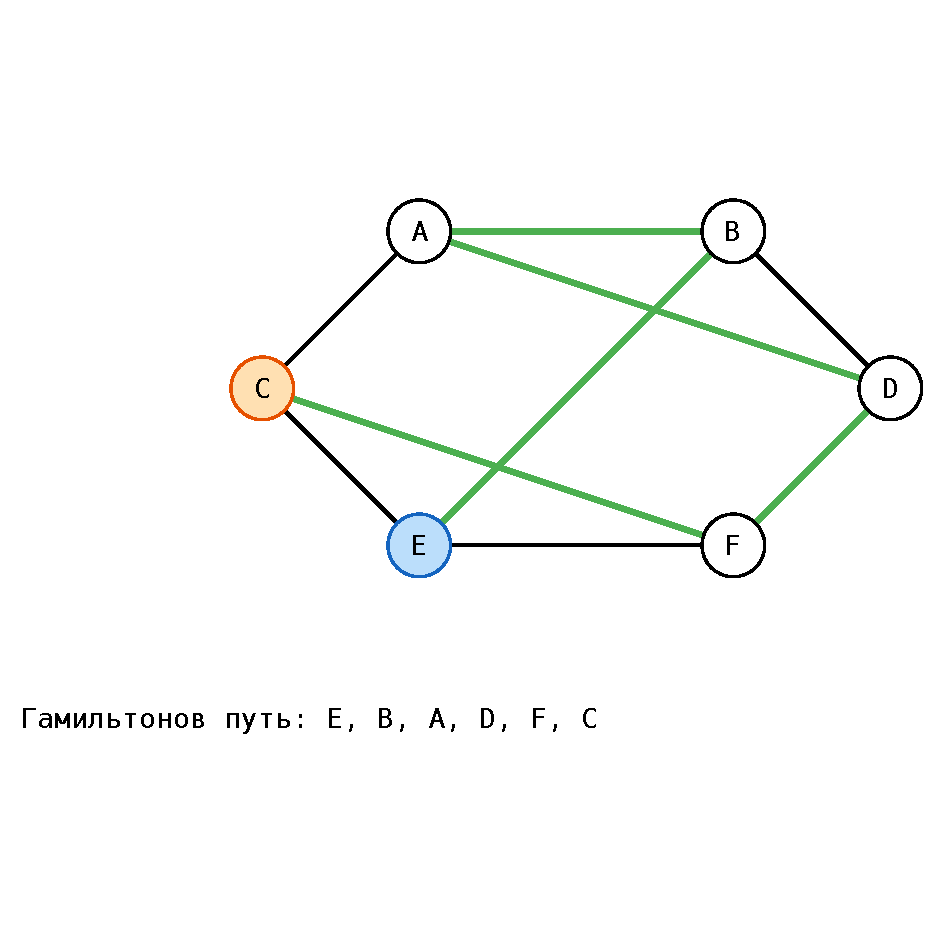
\includegraphics[width=0.46\textwidth]{python/lec06/hamilton/hamilton-2.pdf}\\[2pt]{\scriptsize Шаг 2. Отрезок $(A,B)$ перевёрнут: гамильтонов путь}} &
\shortstack{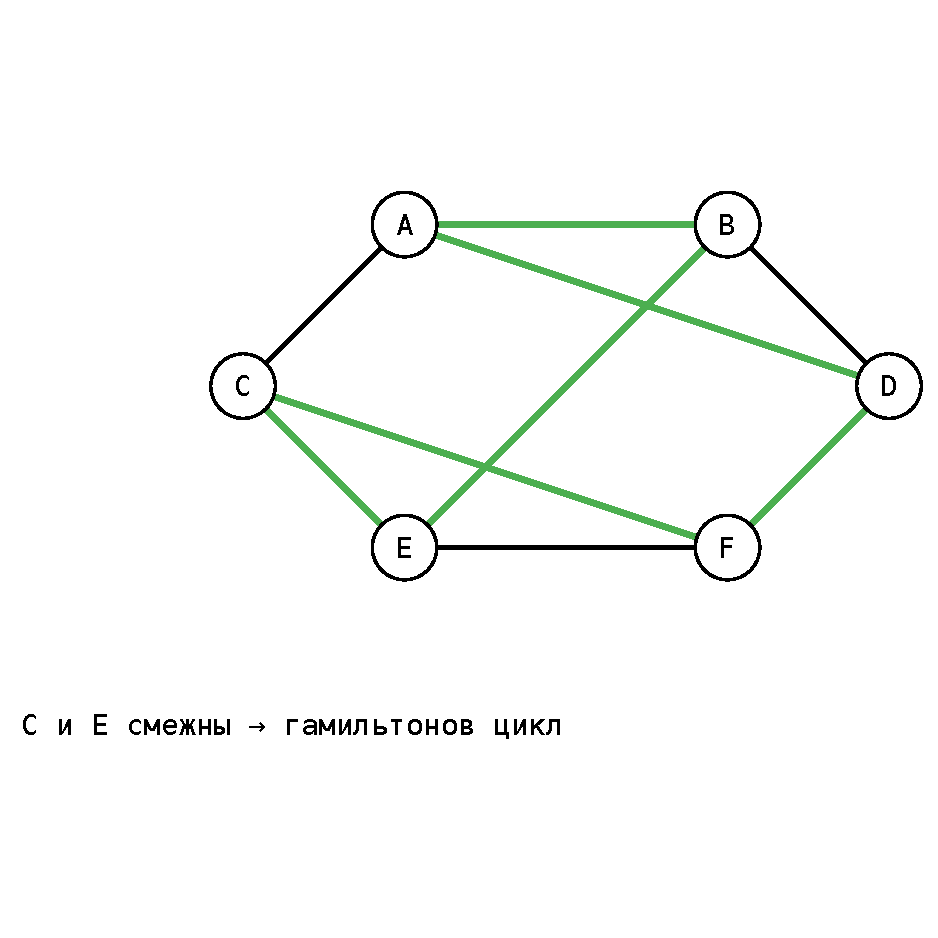
\includegraphics[width=0.46\textwidth]{python/lec06/hamilton/hamilton-3.pdf}\\[2pt]{\scriptsize Шаг 3. $C \sim E$: замыкаем в гамильтонов цикл}} \\
\end{tabular}\end{center}
\end{algo}

% ============================================================
% ГРАФЫ ДЕ БРЁЙНА (стр. 16, dir2 стр. 4)
% ============================================================

\subsection*{Графы де Брёйна}

\begin{defn}{Граф де Брёйна}{de-bruijn}
$\Sigma = \{a_0, \ldots, a_{k-1}\}$ --- алфавит.

$\Sigma^m = \{a_{i_1} \ldots a_{i_m} \mid a_{i_j} \in \Sigma\}$ --- слова длины $m$.

$\Sigma^m = V$ \quad (вершины --- слова длины $m$).

$E = \Sigma^{m+1}$ \quad (рёбра --- слова длины $m+1$).

Ребро $a_{i_1} a_{i_2} \ldots a_{i_m} a_{i_{m+1}}$ соединяет вершину
$(a_{i_1} \ldots a_{i_m})$ с вершиной $(a_{i_2} \ldots a_{i_{m+1}})$:
суффикс первой вершины совпадает с префиксом второй;
$a_{i_1}$ и $a_{i_{m+1}}$ --- любые.

$B(\Sigma, m)$ --- \textbf{граф де Брёйна}.
\end{defn}

\medskip
\noindent\textbf{Пример.}
$\Sigma = \{0, 1\}$, $m = 2$.

% Граф: p16-example-2.graph
\grfig{figures/p16-example-2.pdf}{Граф де Брёйна B(\{0,1\}, 2)}
% Вершины: 00, 01, 10, 11
% Рёбра:
%   00→01 (001), 01→11 (011), 11→10 (110), 10→00 (100)
%   01→10 (010), 10→01 (101)
%   00→00 (000, петля), 11→11 (111, петля)

$\Sigma^2 = \{00, 01, 10, 11\}$ --- вершины.

$B(\{0,1\}, 2)$: рёбра --- все слова длины 3 ($000, 001, 010, 011, 100, 101, 110, 111$).

\medskip
\begin{statement}{Графы де Брёйна всегда эйлеровы}{de-bruijn-euler}
$\forall\, \Sigma$ ($|\Sigma| = k$), $\forall\, m$: граф $B(\Sigma, m)$ ---
эйлеров.
\end{statement}

\begin{proof}
Проверим критерий эйлеровости для ориентированного графа.

\textbf{Полустепени равны.} Из вершины $w = a_{i_1} \ldots a_{i_m}$ выходит
ровно $k$ дуг --- слова $w \cdot a$ для каждой буквы $a \in \Sigma$
(ведут в вершины $a_{i_2} \ldots a_{i_m} a$). Входит в $w$ тоже ровно $k$
дуг --- слова $a \cdot w$ для каждой $a \in \Sigma$. Значит,
$\delta^-(v) = \delta^+(v) = k$ для всех вершин.

\textbf{Связность.} Из любой вершины $u = a_{i_1} \ldots a_{i_m}$ можно
дойти до любой вершины $v = b_{j_1} \ldots b_{j_m}$: последовательно
<<вдвигаем>> буквы слова $v$ справа --- за $m$ шагов
$u \to a_{i_2} \ldots a_{i_m} b_{j_1} \to \ldots \to b_{j_1} \ldots b_{j_m} = v$.
Граф даже сильно связен.

Оба условия критерия выполнены --- эйлеров цикл существует. (Именно он
даёт \emph{последовательность де Брёйна} --- кратчайшую циклическую
строку, содержащую все слова длины $m + 1$.)
\end{proof}

% ============================================================
% ДЕРЕВЬЯ (стр. 16–17, dir2 стр. 4–5)
% ============================================================

\subsection*{Деревья}

\begin{defn}{Дерево}{tree}
Ациклический, связный граф.
\end{defn}

Что знаем:
\begin{enumerate}
  \item $G$ --- дерево $\;\Rightarrow\;$ $|E| = |V| - 1$.
  \item $G$ --- связный, $|E| = |V| - 1$ $\;\Rightarrow\;$ $G$ --- дерево.
  \item $G$ --- дерево $\;\Rightarrow\;$ $\forall\, u, v \in V$: $\exists!\;$ цепь.
  \item Если $|V| \geq 4$ $\;\Rightarrow\;$ дерево, $|V|!$, $|E|!$ --- не единственно!
\end{enumerate}

\medskip
\noindent\textbf{Помеченные / непомеченные деревья.}

Помеченные (3 вершины):
$A$--$B$--$C$,\quad $A$--$C$--$B$,\quad $B$--$A$--$C$.

Непомеченные (3 вершины): $\circ$--$\circ$--$\circ$ \quad (единственное).

% ============================================================
% КОД ПРЮФЕРА (стр. 17, dir2 стр. 5)
% ============================================================

\subsection*{Код Прюфера}

Как компактно закодировать помеченное дерево: \textbf{код Прюфера}.

$G(V, E)$ --- дерево, $|V| = n$.

$|\operatorname{Pruf}(G)| = n - 2$.

\begin{algo}{Код Прюфера (прямая задача)}{prufer-encode}
\textbf{Дано:} $G(V, E)$ --- дерево, $|V| = n$, порядок лексикографический.

\textbf{Выход:} $\operatorname{Pruf}(G) = \{v_{i_1}, \ldots, v_{i_{n-2}}\}$.

\textbf{Шаг (step):} удаление лексикографически минимального листа;
в код записывается его родитель (единственный сосед). Повторяем,
пока не останется $2$ вершины: код имеет длину $n - 2$.

% Граф: p17-pruffer-example-1.graph
\grfig[0.55]{figures/p17-pruffer-example-1.pdf}{Код Прюфера: дерево 11 вершин}
% Вершины: A, B, C, D, E, F, H, J, I, K, L (11 вершин)
% Рёбра: A—B, B—C, C—D, D—E, E—F, D—H, H—J, D—I, B—K, C—L

\medskip
\noindent\textbf{Пример.}
Дерево (11 вершин): $A$--$B$, $B$--$C$, $C$--$D$, $D$--$E$, $E$--$F$,
$D$--$H$, $H$--$J$, $D$--$I$, $B$--$K$, $C$--$L$.
Порядок: $A, B, C, D, E, F, H, I, J, K, L$.

\medskip
По шагам (лист $\to$ в код пишем его соседа):
\begin{enumerate}
  \item листья $\{A, F, I, J, K, L\}$; минимальный $A$, сосед $B$ $\to$ код $(B)$;
  \item минимальный лист $F$, сосед $E$ $\to$ код $(B, E)$;
  \item $E$ стала листом; минимальный лист $E$, сосед $D$ $\to$ $(B, E, D)$;
  \item минимальный лист $I$, сосед $D$ $\to$ $(B, E, D, D)$;
  \item минимальный лист $J$, сосед $H$ $\to$ $(B, E, D, D, H)$;
  \item $H$ стала листом; сосед $D$ $\to$ $(B, E, D, D, H, D)$;
  \item $D$ стала листом; сосед $C$ $\to$ $(B, E, D, D, H, D, C)$;
  \item минимальный лист $K$, сосед $B$ $\to$ $(B, E, D, D, H, D, C, B)$;
  \item $B$ стала листом; сосед $C$ $\to$ $(B, E, D, D, H, D, C, B, C)$;
        остались две вершины $C$ и $L$ --- стоп.
\end{enumerate}

\[
  \operatorname{Pruf}(G) = (B,\; E,\; D,\; D,\; H,\; D,\; C,\; B,\; C),
  \qquad |\operatorname{Pruf}(G)| = 11 - 2 = 9.
\]

\medskip
\noindent\textbf{Работа алгоритма по шагам.} На каждом шаге удаляется
лист с минимальной меткой (оранжевый), в код дописывается его сосед
(синий); удалённые вершины и рёбра показаны серым.

\begin{center}\begin{tabular}{ccc}
\shortstack{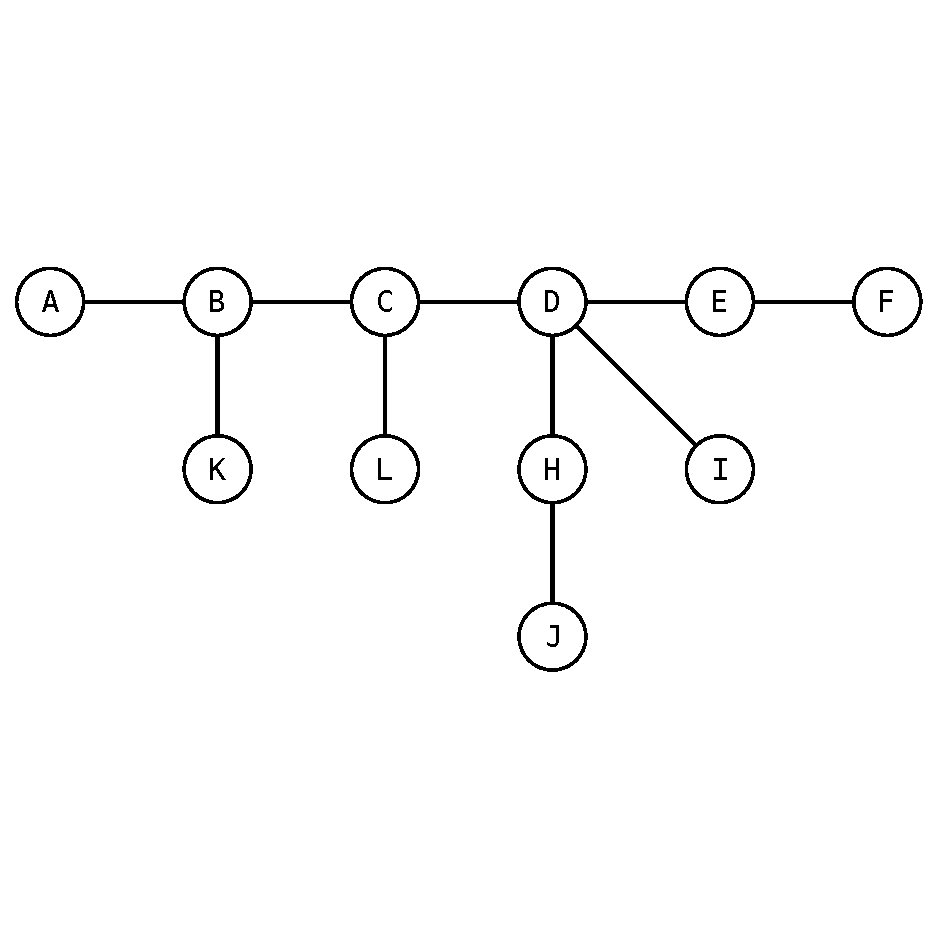
\includegraphics[width=0.28\textwidth]{python/lec06/pruefer/pruefer-0.pdf}\\[2pt]{\scriptsize Шаг 0. Исходное дерево}} &
\shortstack{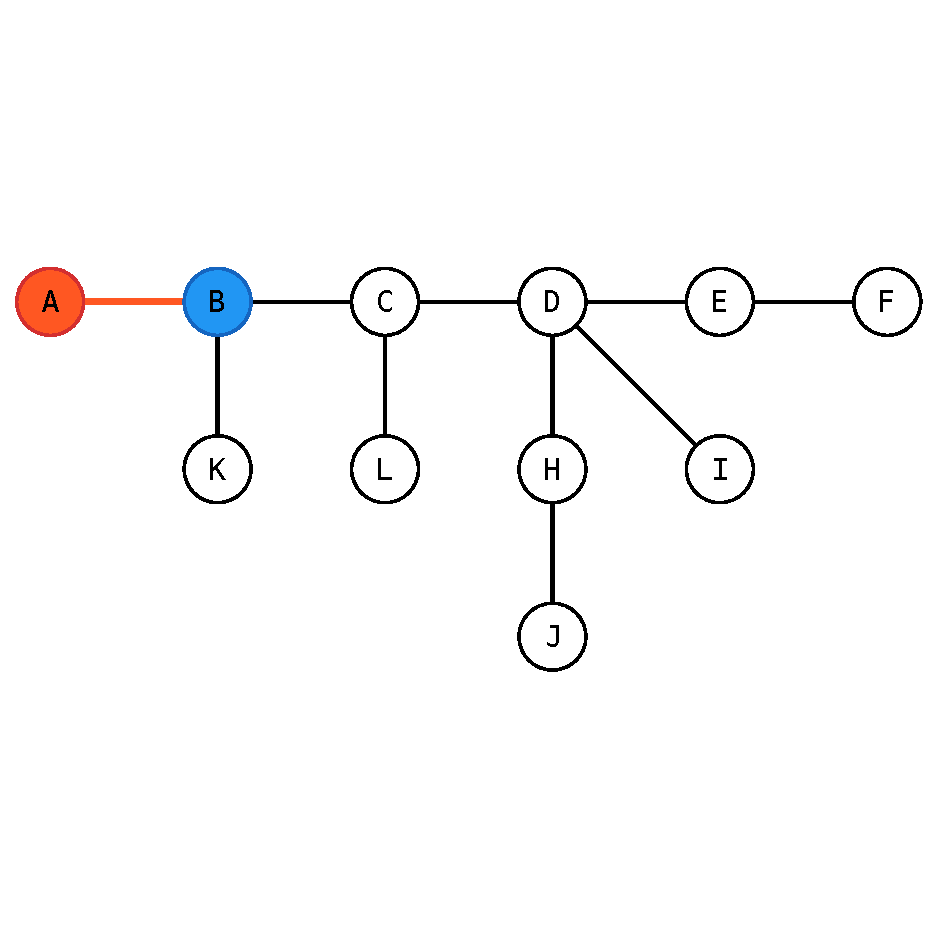
\includegraphics[width=0.28\textwidth]{python/lec06/pruefer/pruefer-1.pdf}\\[2pt]{\scriptsize Шаг 1. $A \to$ код: $B$}} &
\shortstack{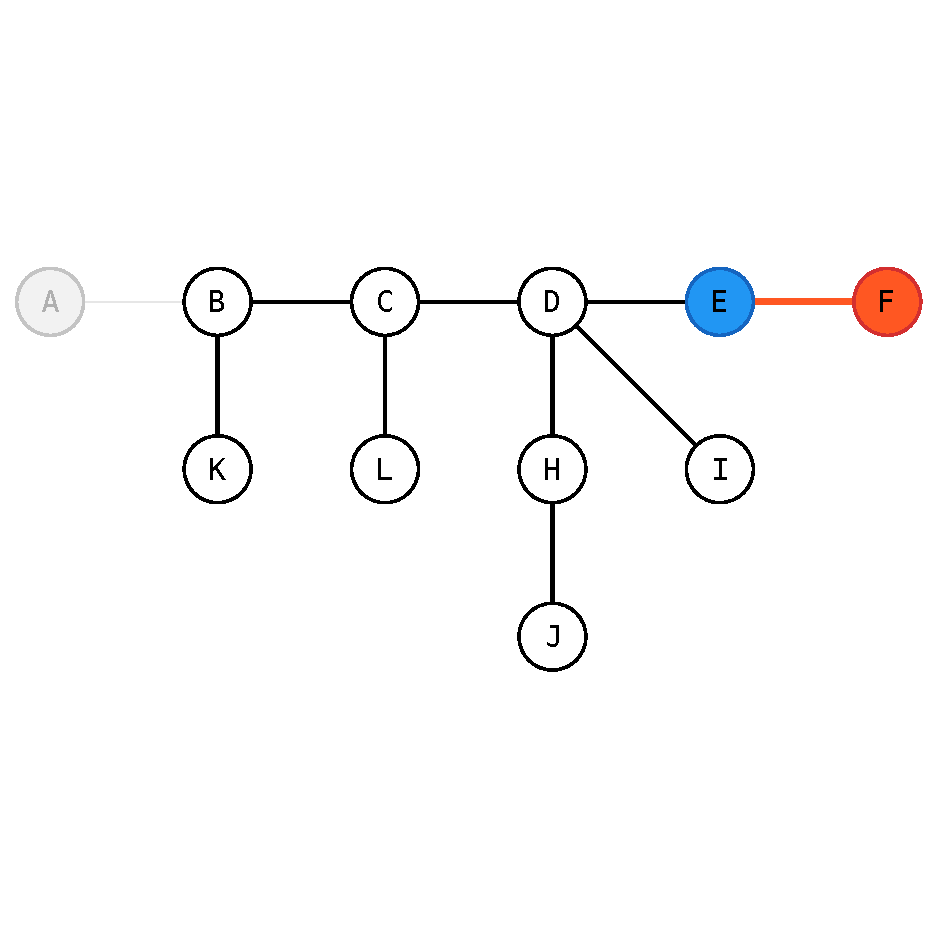
\includegraphics[width=0.28\textwidth]{python/lec06/pruefer/pruefer-2.pdf}\\[2pt]{\scriptsize Шаг 2. $F \to$ код: $E$}} \\
\end{tabular}\end{center}
\begin{center}\begin{tabular}{ccc}
\shortstack{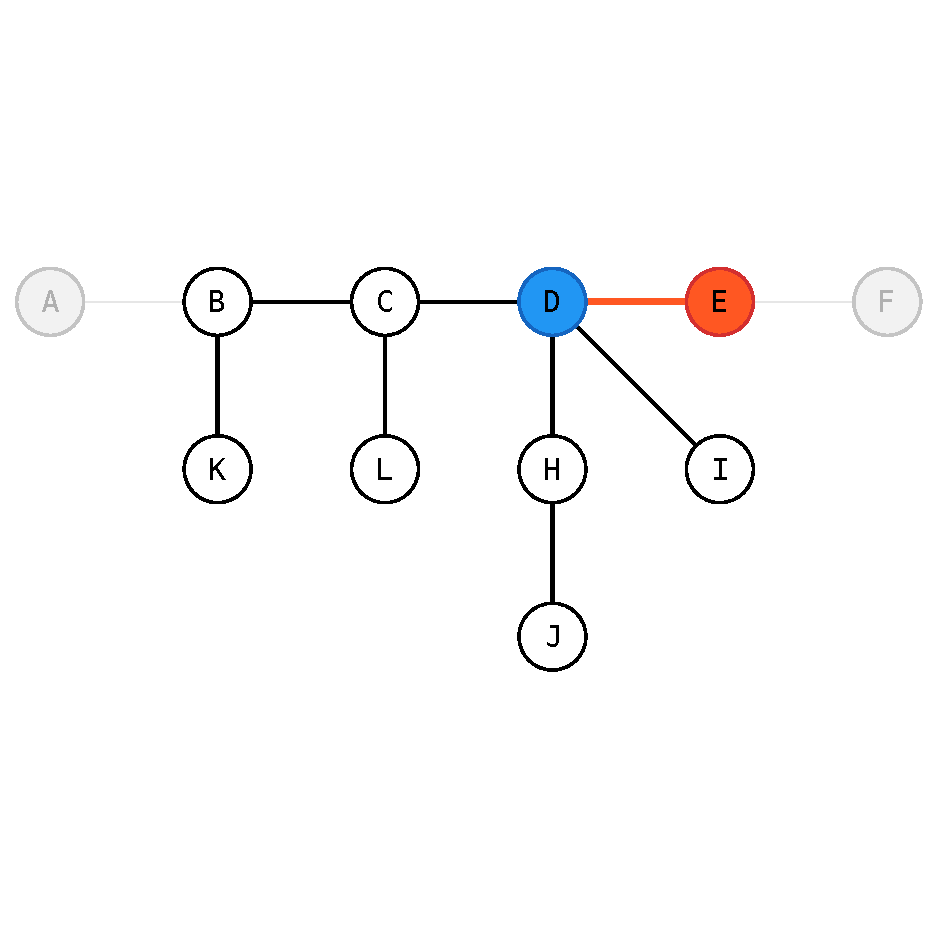
\includegraphics[width=0.28\textwidth]{python/lec06/pruefer/pruefer-3.pdf}\\[2pt]{\scriptsize Шаг 3. $E \to$ код: $D$}} &
\shortstack{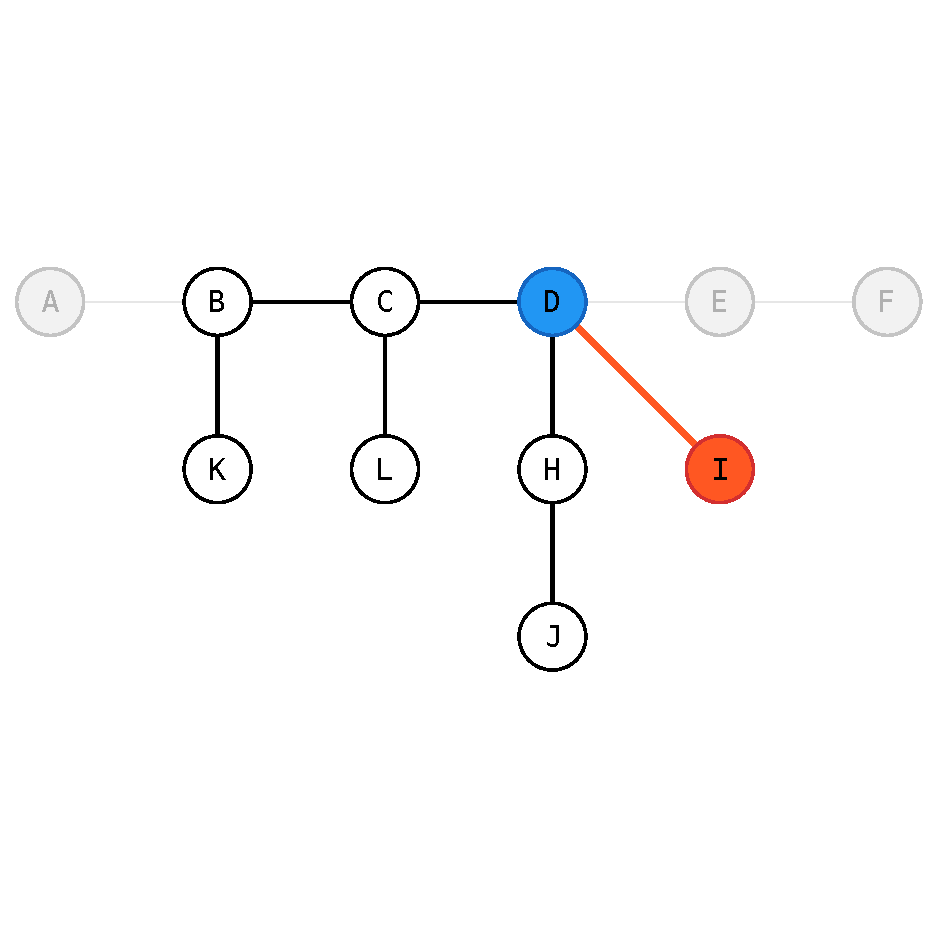
\includegraphics[width=0.28\textwidth]{python/lec06/pruefer/pruefer-4.pdf}\\[2pt]{\scriptsize Шаг 4. $I \to$ код: $D$}} &
\shortstack{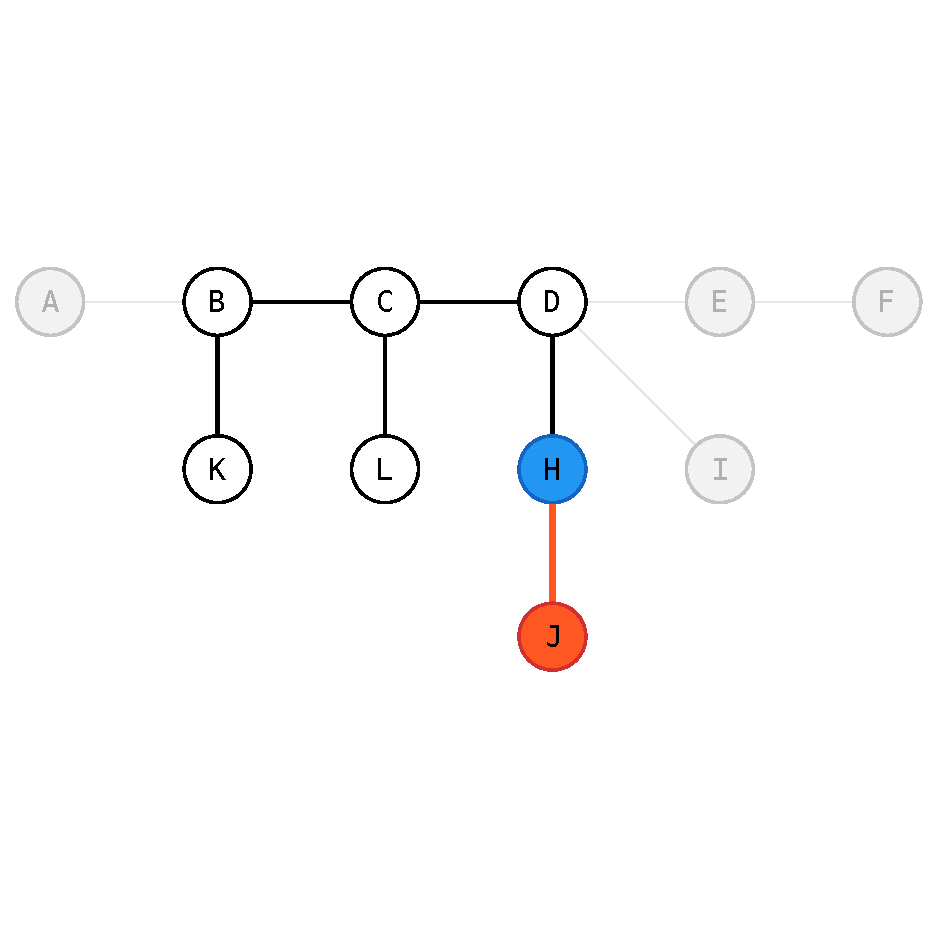
\includegraphics[width=0.28\textwidth]{python/lec06/pruefer/pruefer-5.pdf}\\[2pt]{\scriptsize Шаг 5. $J \to$ код: $H$}} \\
\end{tabular}\end{center}
\begin{center}\begin{tabular}{ccc}
\shortstack{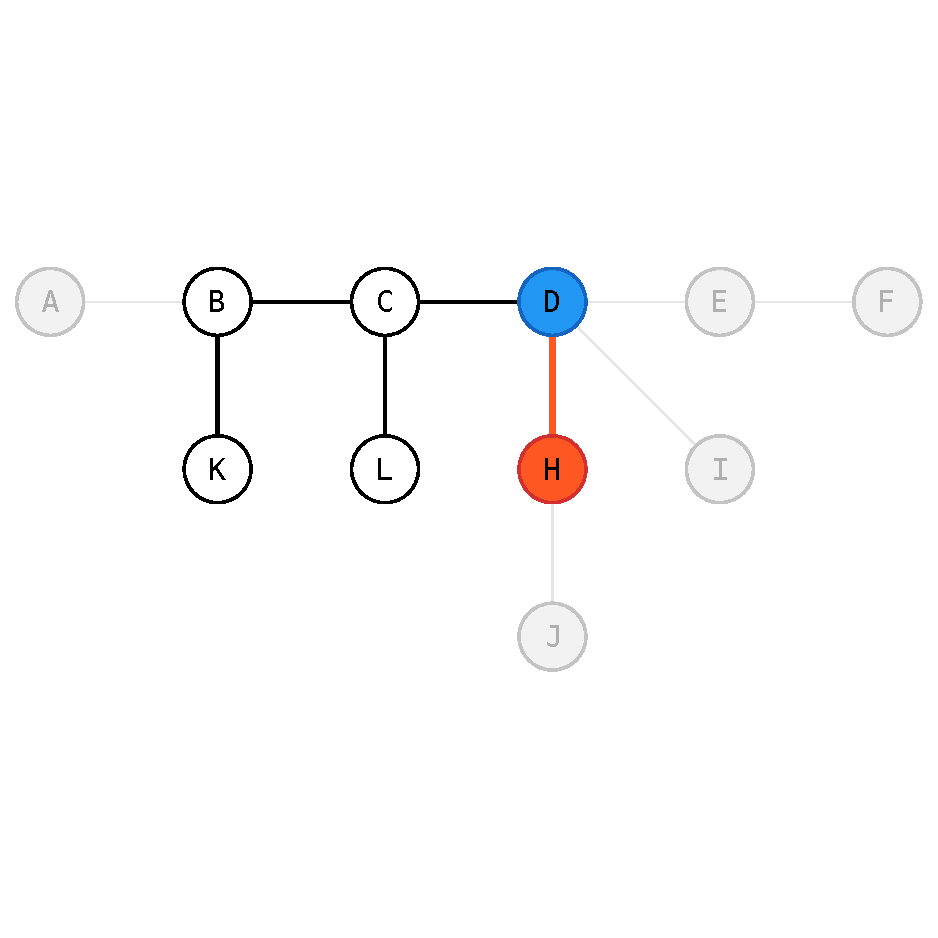
\includegraphics[width=0.28\textwidth]{python/lec06/pruefer/pruefer-6.pdf}\\[2pt]{\scriptsize Шаг 6. $H \to$ код: $D$}} &
\shortstack{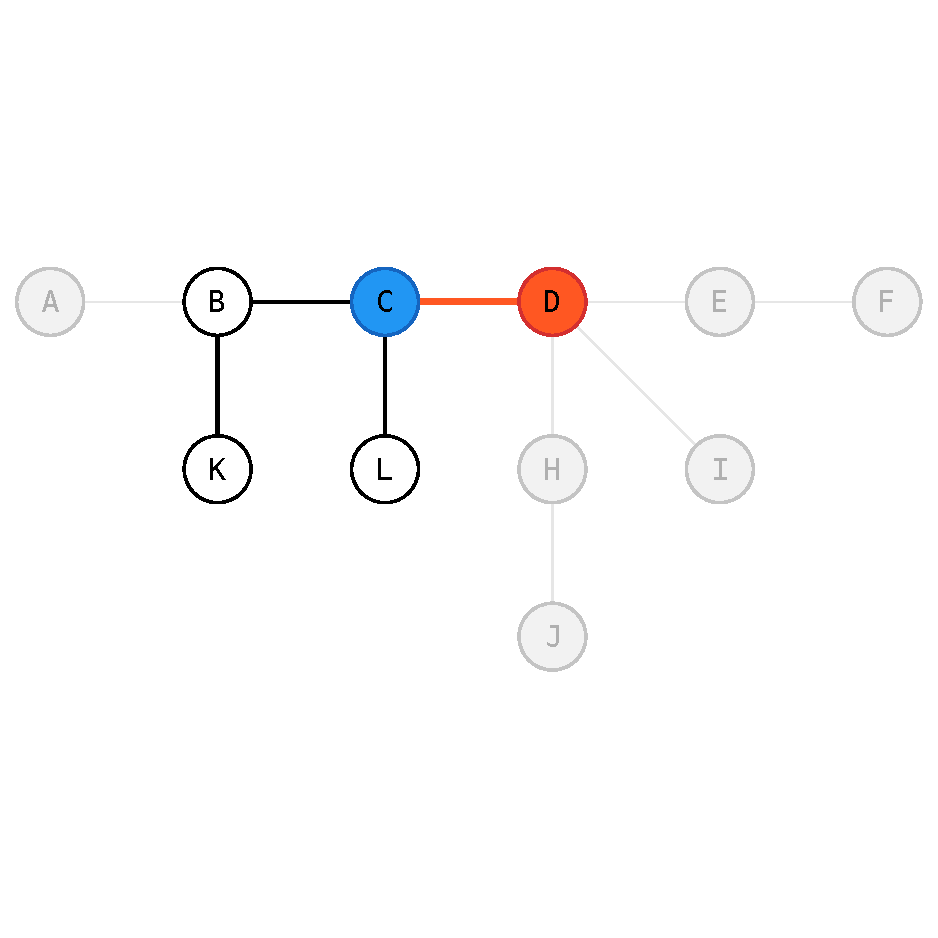
\includegraphics[width=0.28\textwidth]{python/lec06/pruefer/pruefer-7.pdf}\\[2pt]{\scriptsize Шаг 7. $D \to$ код: $C$}} &
\shortstack{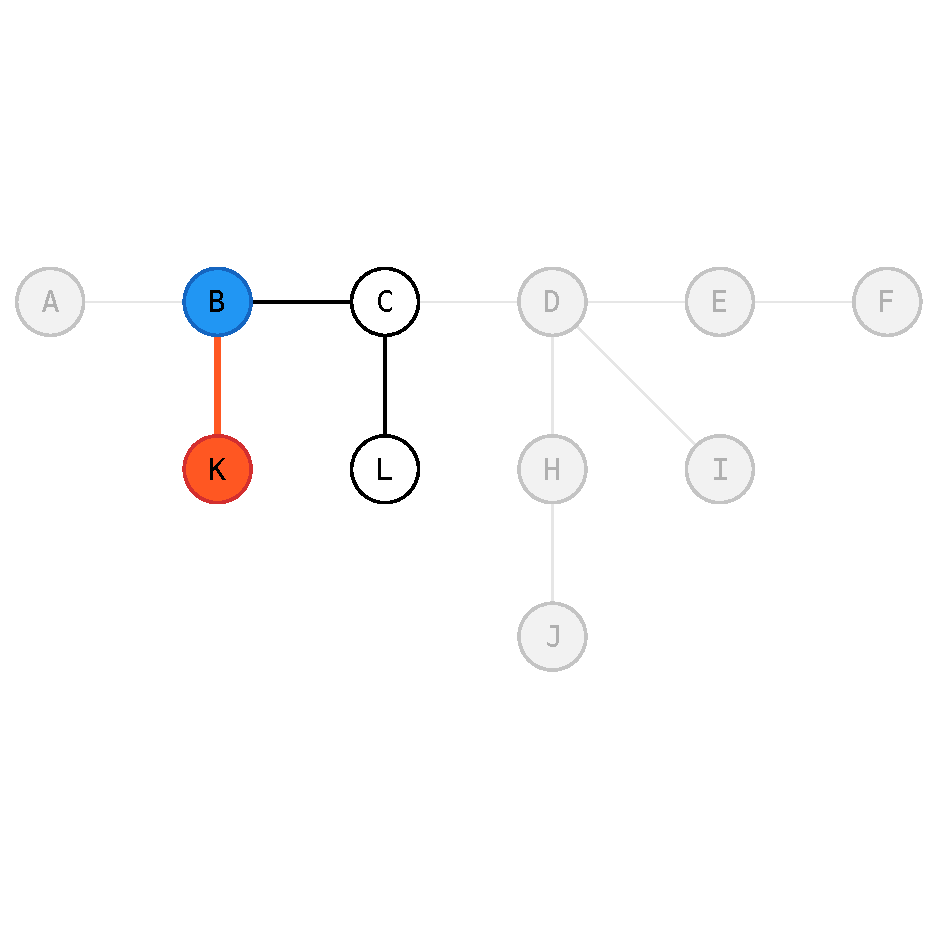
\includegraphics[width=0.28\textwidth]{python/lec06/pruefer/pruefer-8.pdf}\\[2pt]{\scriptsize Шаг 8. $K \to$ код: $B$}} \\
\end{tabular}\end{center}
\begin{center}\begin{tabular}{cc}
\shortstack{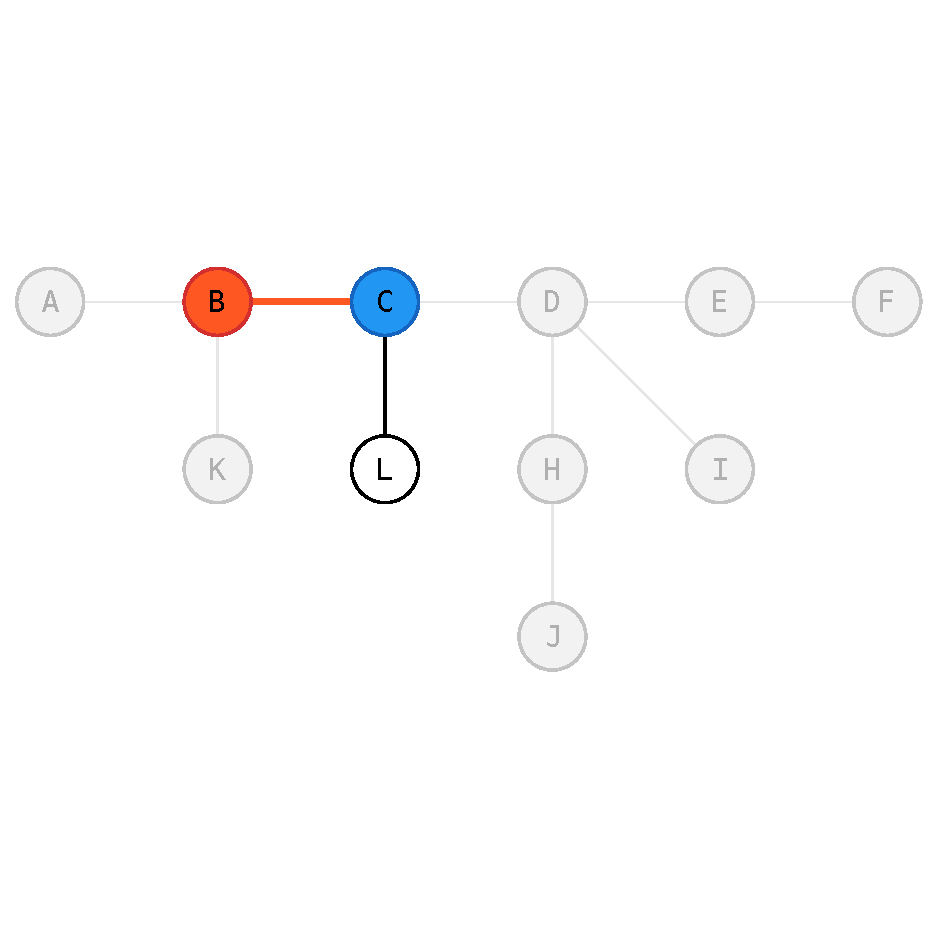
\includegraphics[width=0.28\textwidth]{python/lec06/pruefer/pruefer-9.pdf}\\[2pt]{\scriptsize Шаг 9. $B \to$ код: $C$}} &
\shortstack{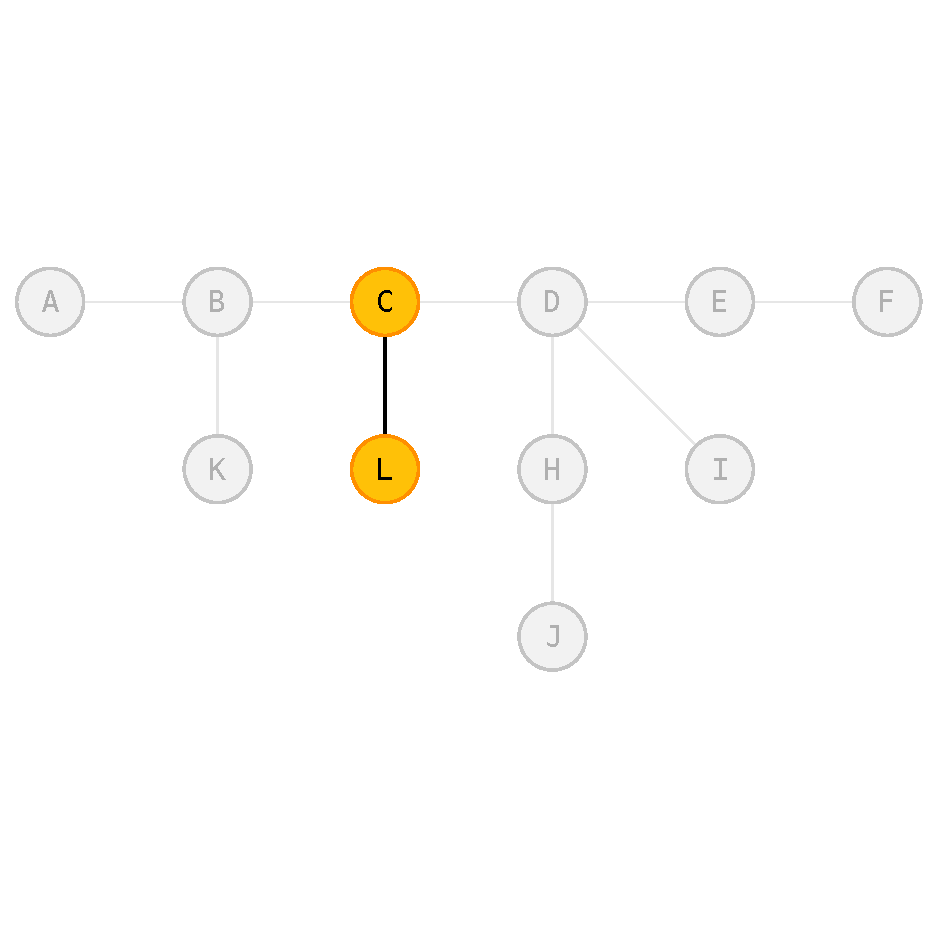
\includegraphics[width=0.28\textwidth]{python/lec06/pruefer/pruefer-10.pdf}\\[2pt]{\scriptsize Шаг 10. Остались $C$ и $L$ --- стоп}} \\
\end{tabular}\end{center}
\end{algo}

% ============================================================
\begin{task}{Код Прюфера: прямая и обратная задача}{pruffer-task}
\textbf{Условие.} \textbf{(а)} Постройте код Прюфера для дерева на вершинах
$1,\dots,6$ с рёбрами $1\!-\!3,\ 2\!-\!3,\ 3\!-\!4,\ 4\!-\!5,\ 4\!-\!6$.
\textbf{(б)} Восстановите дерево по коду Прюфера $(3,3,4,4)$.

\begin{center}
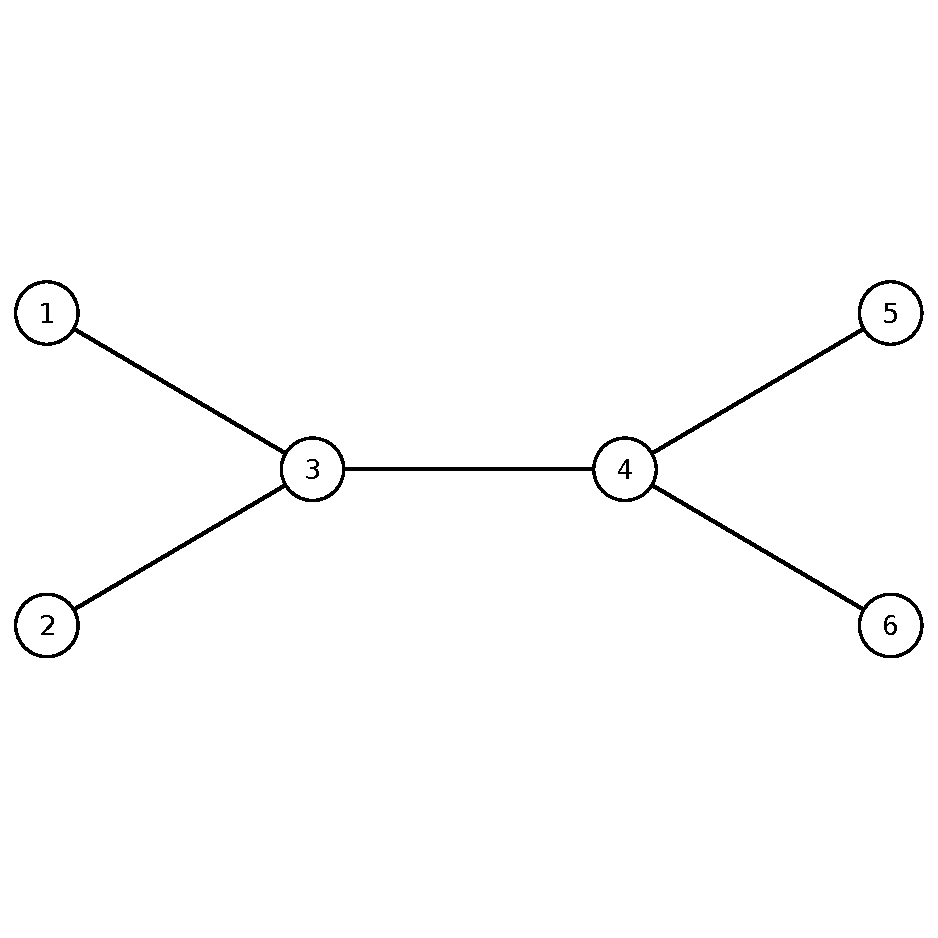
\includegraphics[width=0.45\textwidth]{figures/task-pruefer-1.pdf}
\end{center}

\smallskip
\textbf{Решение (а).} На каждом шаге удаляем лист с наименьшим номером и
записываем номер его единственного соседа; повторяем, пока не останется $2$
вершины (для дерева на $n$ вершинах код имеет длину $n-2=4$).
\begin{enumerate}
  \item Листья $\{1,2,5,6\}$. Наименьший --- $1$, сосед $3$. Записываем $3$.
  \item Листья $\{2,5,6\}$. Наименьший --- $2$, сосед $3$. Записываем $3$.
  \item Теперь $3$ стала листом (соединена только с $4$). Листья $\{3,5,6\}$.
        Наименьший --- $3$, сосед $4$. Записываем $4$.
  \item Листья $\{5,6\}$. Наименьший --- $5$, сосед $4$. Записываем $4$.
        Осталось $2$ вершины ($4$ и $6$) --- стоп.
\end{enumerate}
Код Прюфера: $(3,3,4,4)$.

\smallskip
\textbf{Решение (б).} Обратный алгоритм. Список степеней: каждая вершина
встречается в коде $(\deg-1)$ раз, поэтому степень $=$ (число вхождений в код)
$+1$. Для кода $(3,3,4,4)$ и вершин $1\dots6$:
\[
  \deg 3=3,\ \deg 4=3,\ \deg 1=\deg 2=\deg 5=\deg 6=1.
\]
На каждом шаге берём наименьший лист (вершину степени $1$, не входящую в
оставшийся код) и соединяем с первым элементом кода:
\begin{enumerate}
  \item Код $(3,3,4,4)$; наименьший лист $1$ $\to$ ребро $1\!-\!3$; убираем $3$ из кода.
  \item Код $(3,4,4)$; наименьший лист $2$ $\to$ ребро $2\!-\!3$; убираем $3$.
  \item Код $(4,4)$; теперь $3$ стала листом, наименьший лист $3$ $\to$ ребро $3\!-\!4$; убираем $4$.
  \item Код $(4)$; наименьший лист $5$ $\to$ ребро $5\!-\!4$; убираем $4$.
  \item Код пуст; остались вершины $4$ и $6$ $\to$ ребро $4\!-\!6$.
\end{enumerate}
Восстановленные рёбра: $1\!-\!3,\ 2\!-\!3,\ 3\!-\!4,\ 4\!-\!5,\ 4\!-\!6$ ---
совпадают с исходным деревом из пункта (а) (см. рисунок выше), как и
должно быть.

\textbf{Ответ.} Код Прюфера дерева --- $(3,3,4,4)$; обратное восстановление даёт
то же дерево.
\end{task}

% ============================================================
\begin{task}{Последовательность де Брёйна над алфавитом 0 и 1}{debruijn-task}
\textbf{Условие.} Постройте граф де Брёйна для слов длины $2$ над алфавитом
$\{0,1\}$ и найдите кратчайшую циклическую последовательность, содержащую все
$2$-буквенные слова в качестве подстрок.

\smallskip
\textbf{Решение.} В графе де Брёйна $B(\{0,1\},2)$ вершины --- слова длины $1$
(то есть $0$ и $1$), а дуги --- слова длины $2$: дуга из $u$ в $v$ помечена
словом $uv$. Получаем $4$ дуги:
\[
  0\!\xrightarrow{00}\!0,\quad 0\!\xrightarrow{01}\!1,\quad
  1\!\xrightarrow{11}\!1,\quad 1\!\xrightarrow{10}\!0.
\]

\begin{center}
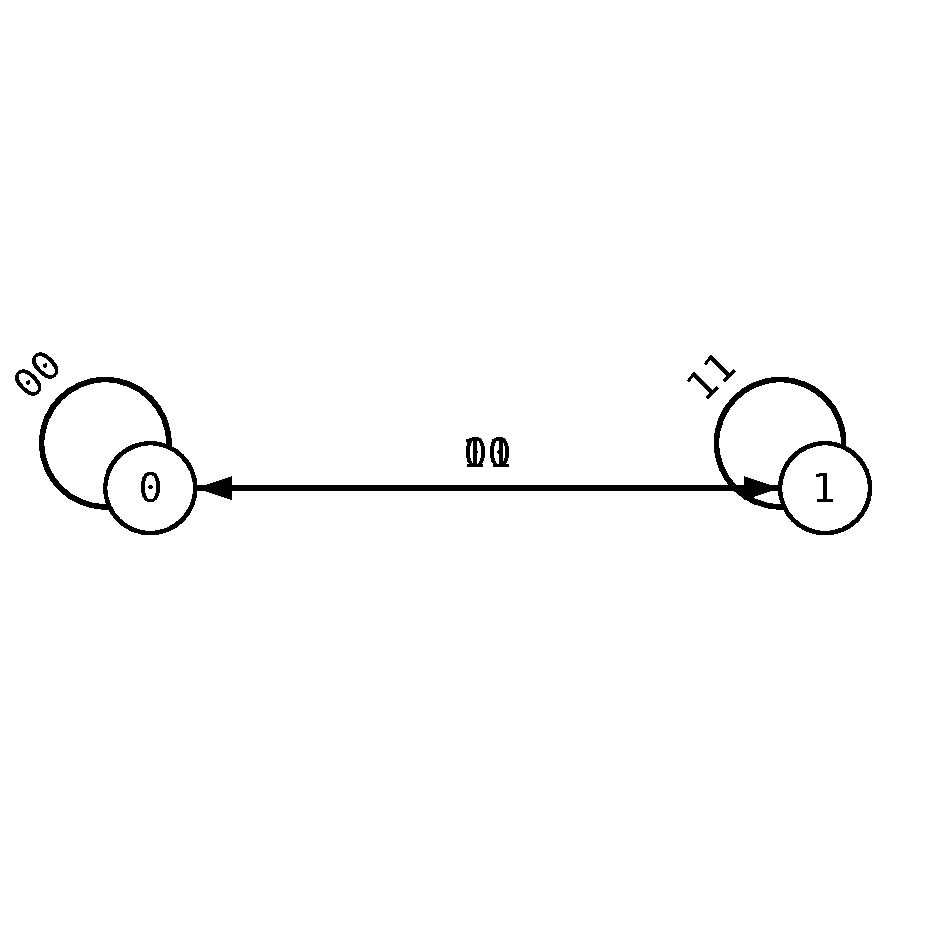
\includegraphics[width=0.35\textwidth]{figures/task-debruijn-1.pdf}
\end{center}
Искомая последовательность --- это \emph{эйлеров цикл} (он проходит по каждой
дуге-слову ровно один раз). У каждой вершины полустепени захода и исхода равны
$2$, граф связен --- эйлеров цикл существует. Один из них:
\[
  0\xrightarrow{00}0\xrightarrow{01}1\xrightarrow{11}1\xrightarrow{10}0,
\]
что даёт циклическую последовательность $\mathbf{0011}$. Читая её по кругу,
получаем все $2$-буквенные слова: $00,\ 01,\ 11,\ 10$.

\textbf{Ответ.} Кратчайшая циклическая последовательность --- $0011$ (длина
$4=2^2$), содержит все четыре слова длины $2$.
\end{task}

% ============================================================
\begin{task}{Гамильтоновость: теорема Дирака}{dirac-task}
\textbf{Условие.} Граф на $5$ вершинах $A,B,C,D,E$ задан как полный граф $K_5$
без двух рёбер $AD$ и $BE$. Является ли он гамильтоновым? Постройте
гамильтонов цикл.

\begin{center}
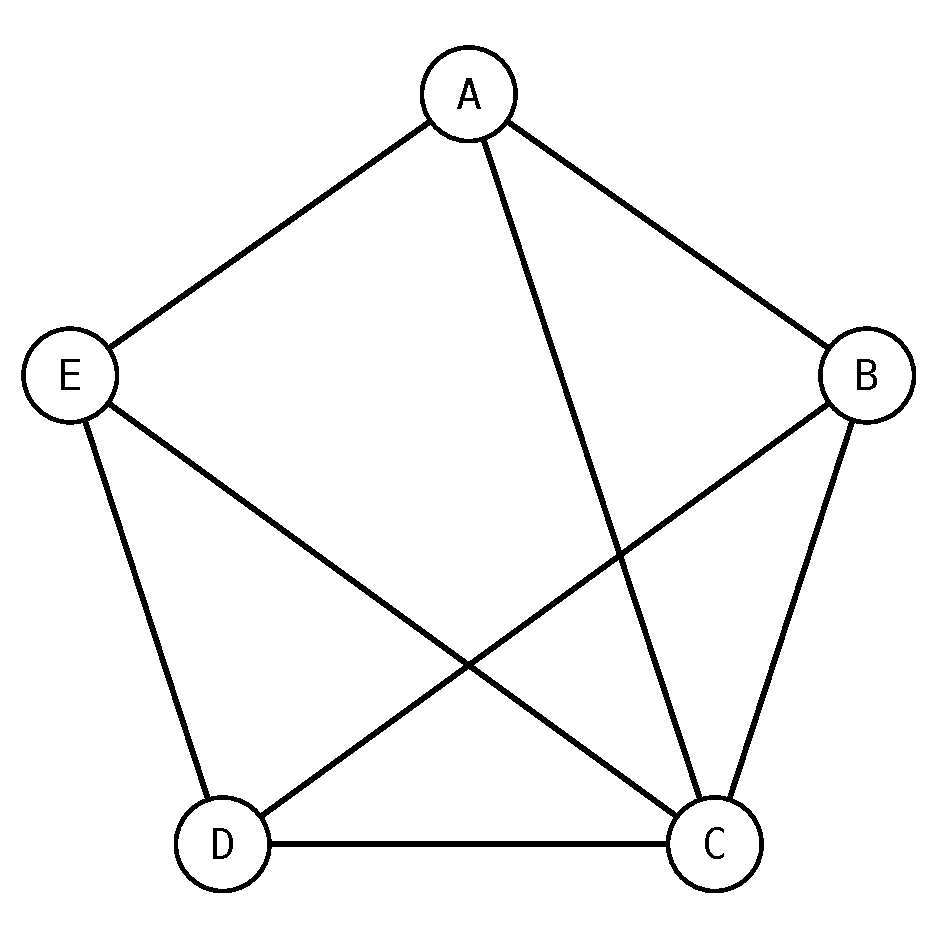
\includegraphics[width=0.35\textwidth]{figures/task-dirac-1.pdf}
\end{center}

\smallskip
\textbf{Решение.} Теорема Дирака: если в графе на $n\geq 3$ вершинах степень
каждой вершины не меньше $n/2$, то граф гамильтонов. Здесь $n=5$, порог
$n/2=2{,}5$. Подсчитаем степени (в $K_5$ каждая вершина имела степень $4$;
удаление $AD$ и $BE$ уменьшает на единицу степени $A,D,B,E$):
\[
  \deg A=\deg B=\deg D=\deg E=3,\qquad \deg C=4.
\]
Все степени $\geq 3>2{,}5$, поэтому по теореме Дирака граф гамильтонов.

Построим гамильтонов цикл, обходя все вершины по одному разу и избегая
отсутствующих рёбер $AD,BE$:
\[
  A\!-\!B\!-\!D\!-\!C\!-\!E\!-\!A.
\]
Проверим рёбра: $AB,\ BD,\ DC,\ CE,\ EA$ --- все присутствуют (среди них нет ни
$AD$, ни $BE$).

\begin{center}
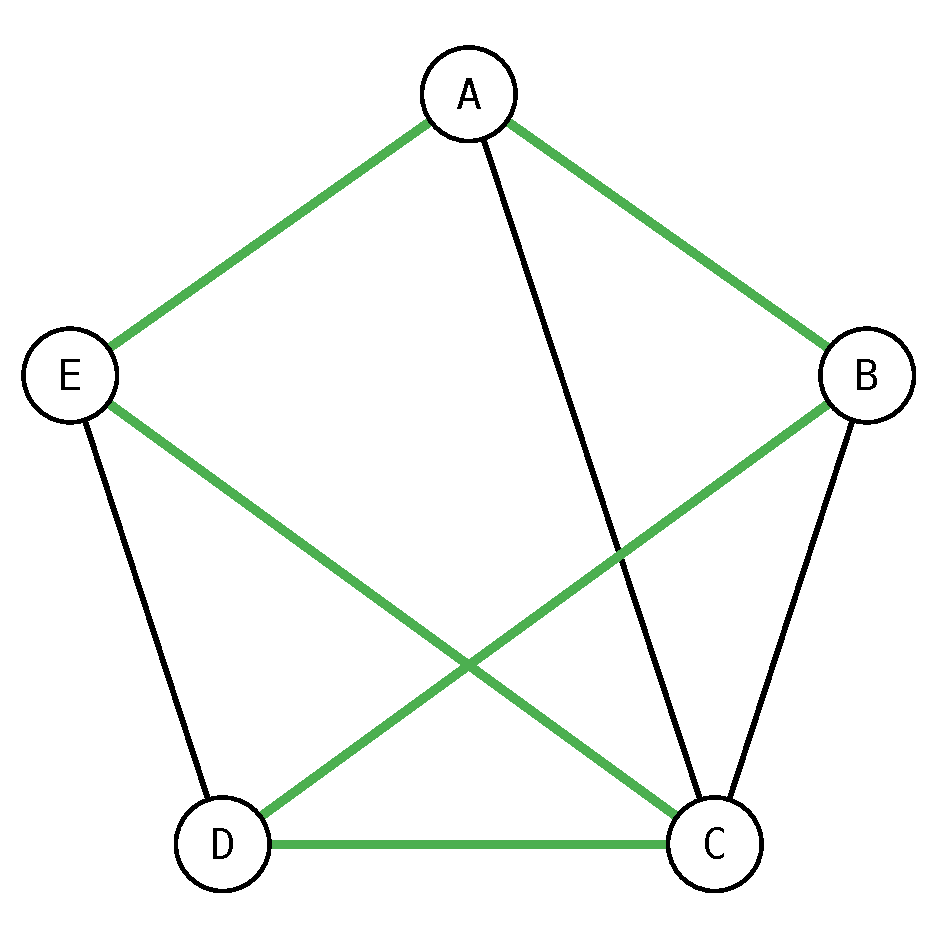
\includegraphics[width=0.35\textwidth]{figures/task-dirac-2.pdf}
\end{center}

\textbf{Ответ.} Граф гамильтонов (условие Дирака выполнено); гамильтонов цикл
$A\!-\!B\!-\!D\!-\!C\!-\!E\!-\!A$.
\end{task}
